\chapter{\ifproject%
\ifenglish Project Structure and Methodology\else โครงสร้างและขั้นตอนการทำงาน\fi
\else%
\ifenglish Project Structure\else โครงสร้างของโครงงาน\fi
\fi
}

ในบทนี้จะกล่าวถึงโครงสร้างของระบบในภาพรวม และขั้นตอนการทํางานของระบบ โดยขั้นตอนการทํางาน \\
จะแบ่งเป็น 2 ส่วนใหญ่ ๆ คือส่วนของโมดูลกล้องและเซิร์ฟเวอร์

\makeatletter

% \renewcommand\section{\@startsection {section}{1}{\z@}%
%                                    {13.5ex \@plus -1ex \@minus -.2ex}%
%                                    {2.3ex \@plus.2ex}%
%                                    {\normalfont\large\bfseries}}

\makeatother
%\vspace{2ex}
% \titleformat{\section}{\normalfont\bfseries}{\thesection}{1em}{}
% \titlespacing*{\section}{0pt}{10ex}{0pt}

\section{ภาพรวมโครงสร้างและการทำงานของระบบ}


\begin{figure}[h]
  \begin{center}
    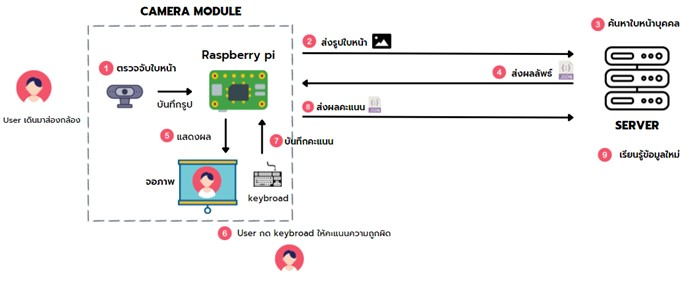
\includegraphics{pic/overview.jpg}
  \caption[Poem]{Flow Diagram ภาพรวมของระบบ}
  \end{center}
  \label{fig:overview}
\end{figure}

\subsection{โมดูลกล้อง (Camera Module)}

\begin{figure}[h]
  \begin{center}
    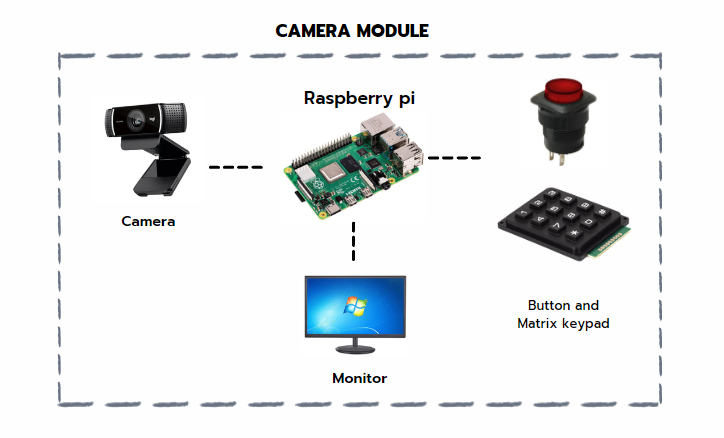
\includegraphics[scale=.6]{pic/camera.png}
    \caption[Poem]{ส่วนประกอบต่าง ๆ ที่ใช้ในโมดูลกล้อง (Camera Module)}
    \label{fig:camera}
  \end{center}
\end{figure}
\newpage
อุปกรณ์ที่ใช่ในโมดูลกล้องสำหรับการตรวจจับใบหน้า มีดังนี้
\begin{enumerate}
  \item Raspberry Pi 4 Model B : แพลตฟอร์มที่ใช้ในการค้นหาใบหน้าบุคคล ซึ่งคุณสมบัติที่จำเป็นได้แก่ 
  มีขนาดเล็ก สามารถส่งข้อมูลผ่านเครื่องข่ายไร้สายไวไฟ (WI-FI) หรือผ่านเครือข่ายที่ใช้สาย (LAN) สามารถอ่านข้อมูลภาพจากกล้องถ่ายภาพ 
  และส่งรูปภาพไปยังเซิร์ฟเวอร์และรอรับผลลัพธ์ และส่งผลลัพธ์จากปุ่มกลับไปยังเซิร์ฟเวอร์
  \item Camera : กล้องเว็บแคมที่มีใช้มาการส่งภาพใบหน้าไปยัง Raspberry Pi
  \item Monitor : หน้าจอแสดงผลที่ใช้ในการแสดงผลลัพธ์ของการระบุตันตน
  \item Button และ Matrix keypad : ใช้ในการรับการให้คะแนนการแสดงผลลัพธ์และแก้ไขความถูกผิดของการแสดงผลลัพธ์
\end{enumerate}

\subsection{การส่งข้อมูลไปยังเซิร์ฟเวอร์}
การส่งรูปภาพจากโมดูลกล้องไปยังเซิร์ฟเวอร์นั้นในโมดูลกล้องใช้คำสั่ง ภาษาไพธอน (Python) ในการใช้สั่งคำส่งของระบบ (System)
คือเคิร์ล  (Client for URLs: cURL) ในการส่งรูปภาพผ่าน HTTP ไปยังเซิร์ฟเวอร์ที่เป็น (RESTful Web Services: RWS)
ผ่านเลขที่อยู่ไอพี (IP Address) ของเซิร์ฟเวอร์ โดย RWS นั้นใช้ Flask Framework 
ในการสร้างเนื่องจาก Flask Framework นั้นใช้ภาษาไพธอน (Python) ในการเขียนทำให้มีความสะดวกในการเรียก TensorFlow และ OpenCV มาใช้งาน

\subsection{การแสดงผลการระบุตัวตน}
การแสดงผลที่หน้าจอที่เชื่อมต่อกับ Raspberry Pi โดยรับข้อมูลมาจากเซิร์ฟเวอร์ที่ส่งข้อมูลบุคคลที่มีความใกล้เคียงจำนวน 5 คน 
แต่จะต้องมีความใกล้เคียงกับรายชื่อในฐานข้อมูลมากกว่า 80 เปอร์เซ็นต์จึงจะส่งผลลัพธ์ได้ แต่ถ้าไม่มีความใกล้เคียงมากกว่า 80 เปอร์เซ็นต์ก็จะแสดงผลว่าไม่รู้จัก 
โดยเซิร์ฟเวอร์ส่งข้อมูลแบบ JSON กลับมาให้ Raspberry Pi แบบการสนอง (Response) เมื่อรับข้อมูลจากเซิร์ฟเวอร์จะทำการนำไปแสดงผลที่หน้าจอ 
และเมื่อให้คะแนนความถูกผิดแล้วนั้นจะส่งผลคะแนนกลับไปยังเซิร์ฟเวอร์เพื่อทำการย้ายไปยังที่จัดเก็บตามรายชื่อ \\

\begin{figure}[h]
  \begin{center}
    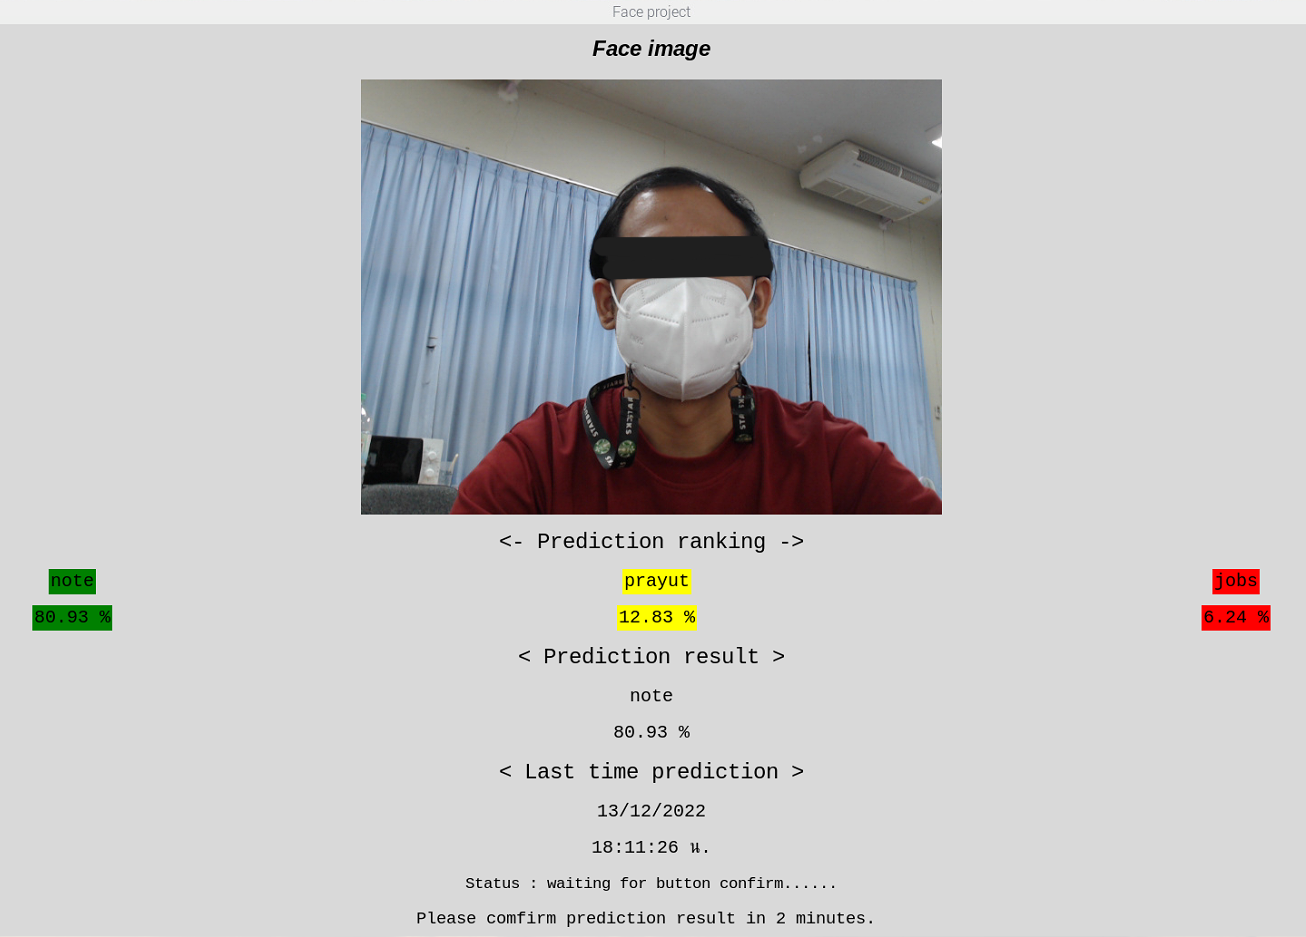
\includegraphics[scale=.45]{pic/result_page_blind.png}
  \caption[Poem]{แสดงผลลัพธ์การระบุตัวตน}
  \end{center}
  \label{fig:predict_result}
\end{figure}
\newpage

\subsection{เซิร์ฟเวอร์ (Server)}
ทำหน้าที่ในการเป็นเว็ปเซอร์วิส (Web service) ในการรับรูปภาพเพื่อนำรูปภาพมาระบุตัวตนโดยใช้ OpenCV
เพื่อบอกว่ารูปนี้มีความใกล้เคียงกับบุคคลโดยโมเดลที่ใช้ในการระบุตัวตนนั้นมาจาก TensorFlow ในการนำรูปภาพจากที่จัดเก็บ (Storage) 
มาทำการเรียนรู้จนได้โมเดลไปใช้งานและเมื่อ OpenCV บอกผลลัพธ์ได้แล้วจึงทำการส่งขอร้อง (Request) 
กลับไปยังโมดูลกล้องแล้วทำการรอรับคะแนนเพื่อที่จะนำรูปภาพย้ายไปยังตำแหน่งที่จัดเก็บของบุลคลนั้น ๆ เมื่อจบวันในทุก ๆ 
วันเซิร์ฟเวอร์จะทำการสั่ง TensorFlow เรียนรู้รูปภาพใหม่และนำโมเดลใหม่ไปใช้งาน โดยตัวเซิร์ฟเวอร์จะมีความต้องการด้านฮาร์ดแวร์คือต้องมีความจุมากกว่า 1 เทราไบต์  (Terabyte) 
หน่วยความจำขนาด 16 จิกะไบต์ (Gigabyte) ในการประมวลผล

\subsection{การระบุตัวตน}
การระบุตัวตนจะใช้ภาพถ่ายใบหน้าที่ได้รับมาจากโมดูลกล้อง โดยใช้ OpenCV ในการระบุตัวตนโดยรับตัวโมเดลที่ใช้ในการทำนายรูปภาพใบหน้าว่ามีความใกล้เคียงมากน้อยเพียงใด
แล้วจึงทำการคัดกรองรูปภาพที่มีความใกล้เคียงกับฐานข้อมูลมากกว่า 80 เปอร์เซ็นต์จึงจะส่งข้อมูลไปให้เซิร์ฟเวอร์ทำการส่ง 
แต่เมื่อไม่มีรูปภาพที่มีความใกล้เคียงกับฐานข้อมูลมากกว่า 80 เปอร์เซ็นต์ ก็จะส่งไปบอกเซิร์ฟเวอร์ว่า "ไม่รู้จักบุคคลนี้"

\subsection{การจัดเก็บรูปภาพใบหน้า}
จัดเก็บรูปภาพใบหน้าลงในที่เก็บข้อมูลในเครื่อง (Local storage) บนเซิร์ฟเวอร์โดยแบ่งเป็นแฟ้มข้อมูล \\(Folder) 
ในแต่ละแฟ้มก็จะเป็นรายชื่อของบุคคลที่ลงทะเบียนหรือเป็นผู้ที่ใช้งานห้อง 
โดยเมื่อได้รับคะแนนจากการระบุตัวตนก็ไปเช็คกับผลลัพธ์จากการระบุแล้วจึงจะย้ายรูปภาพไปยังแฟ้มของรายชื่อนั้น ๆ

\begin{figure}[h]
  \begin{center}
    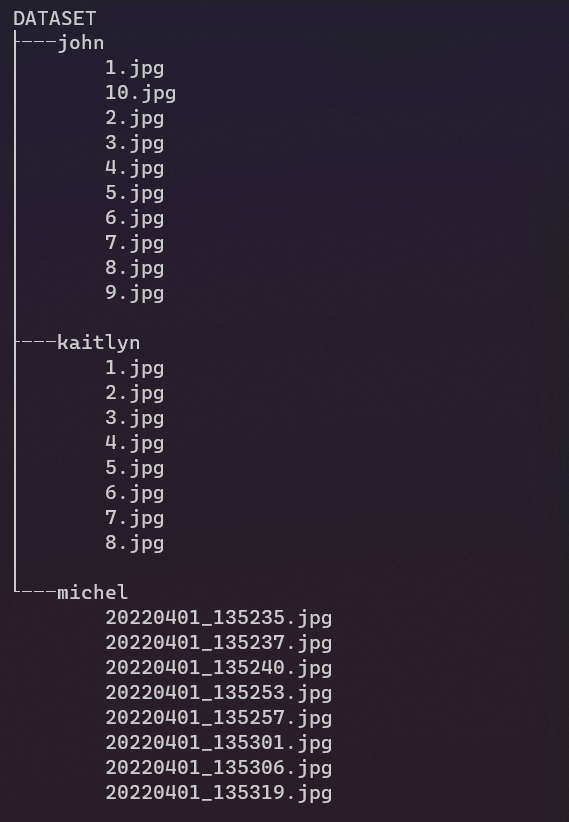
\includegraphics[scale=.5]{pic/dataset.png}
  \caption[Poem]{แผนภาพแสดงการจัดเก็บรูปภาพใบหน้า}
  \end{center}
  \label{fig:folder}
\end{figure}
\newpage

\subsection{การเรียนรู้รูปภาพ}
ใช้ OpenFace ในการเรียนรู้รูปภาพ โดย OpenFace นั้นใช้ภาษาไพธอน (Python) ในการเขียนโปรแกรมเพื่อเรียนรู้รูปภาพใบหน้า เริ่มจากการนำรูปภาพของบุคคลที่บันทึกไว้ในที่จัดเก็บ (Storage) 
และรายชื่อของบุคคลที่มีรูปภาพใบหน้าในที่จัดเก็บ (Storage) แล้วทำการเรียนรู้ด้วย OpenFace จะได้โมเดลการเรียนรู้เพื่อนำไปใช้ในการระบุตัวตนของบุคคล 
โดยขั้นตอนการเรียรรู้จะใช้เวลาขึ้นอยู่กับจำนวนของรูปภาพที่จัดเก็บไว้และใช้ทรัพยากรในการเรียนรู้รูปภาพใบหน้าที่สูงจึงนำ OpenFace ไปทำการเรียนรู้ที่เซิร์ฟเวอร์

% do with it:---it was the black kitten's fault entirely~\cite{aiw}.  For the
